\documentclass{article}

\usepackage[T2A]{fontenc} % Кодировка шрифта
\usepackage[utf8]{inputenc} % Кодировка ввода
\usepackage[english,russian]{babel} % Языковые настройки
\usepackage{graphicx} % Для вставки изображений
\usepackage{amsmath} % Для использования математических формул
\usepackage{amssymb}
\usepackage{cancel}
\usepackage{tikz}
\usepackage{amsfonts} % Для использования математических символов и шрифтов
\usepackage{titlesec} % Для настройки заголовков разделов
\usepackage{titling} % Для настройки титульной страницы
\usepackage{geometry} % Для настройки размеров страницы
\usepackage{pgfplots}
\usepackage{mdframed} % Для создания рамок

\pgfplotsset{compat=1.9}

% Настройка заголовков разделов
\titleformat{\section}
{\normalfont\Large\bfseries}{\arabic{section}}{1em}{}
\titleformat{\subsection}
{\normalfont\large\bfseries}{}{1em}{}

% Настройка титульной страницы
\setlength{\droptitle}{-3em} % Отступ заголовка
\title{\vspace{-1cm}Контрольная работа №6, задание 2}
\author{Вершинин Данил Алексеевич}
\date{\today}

% Настройка размеров страницы
\geometry{a4paper, margin=2cm}

\begin{document}
	\maketitle
	\subsection{Условие}
	Для нахождения положительного корня нелинейного уравнения $x^6-5x-2=0$ предложен метод простой итерации. Исследовать этот метод и сделать выводы о целесообразности его использования.
	
	$$x_{n+1} = \sqrt[6]{5x_n+2}$$.
	\subsection{Решение}
	Пусть $\phi (x) = \sqrt[6]{5x_n+2}$, что является предложенным методом простой итерации. $\phi(x)\in C^1(\mathbb{R_+})$\newline
	\begin{mdframed}
		Проверим выполнение теоремы 1 (см "нелин уравн+итерац.процесс", конспекты лекций). Её условие следующее:
		\[\text{Если функция $\phi(x)$ удовлетворяет условию Липшица с константой $q<1$:}\]
		\[|\phi(x) - \phi(y)|<q|x-y|\]
		\[\text{То метод простой итерации сходится и справедлива оценка}\]
		\[|x_{n+1} - x^*| < q|x_n-x^*|\]
		\[|x_{n+1} - x^*| < q^n|x_0-x^*|\]
		\[|\phi(x)'| \le q < 1\]
	\end{mdframed}
	\begin{figure}[h]
		\centering
		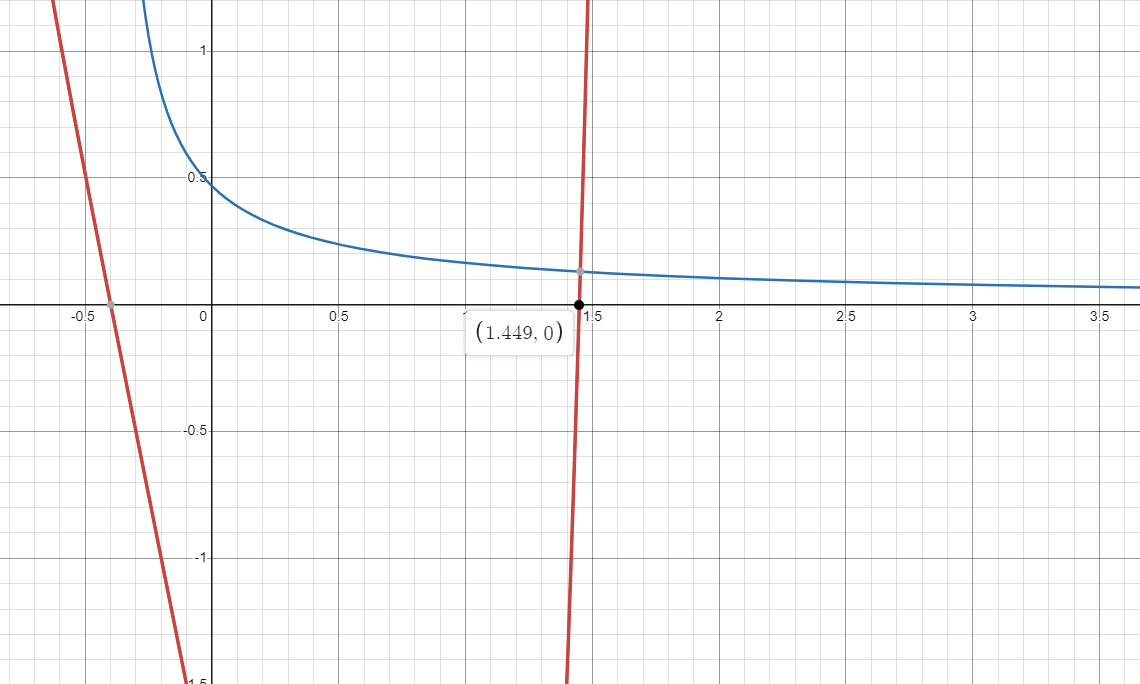
\includegraphics[width=150mm,scale=0.6]{iterations2_1.png}
		\caption{функция из уравнения (красный). Производная предложенного метода (синий)}
	\end{figure}
	
	Проверим нашу функцию $\phi(x)$:
	\[\phi(x) = \sqrt[6]{5x+2}\]
	\[|\phi'(x)| = |\frac{5}{6(5x+2)^{5/6}}|<1\]
	Заметим (*), что модуль можно опустить, т. к. для положительных чисел $\phi'(x)$ всегда положительна, кроме того, асимптотически стремится к 0, при $x\rightarrow\infty$
	\[\frac{5}{6} \cdot \frac{1}{(5x+2)^{5/6}} < 1 \Rightarrow \frac{5}{6} < (5x+2)^{5/6}\Rightarrow x > \frac{(5/6)^{(6/5)} - 2}{5} \approx -0.239\Rightarrow \forall x \in \mathbb{R_+} :|\phi'(x)|<1 \eqno (*)\]	
	Отсюда получаем, что теорема 1 выполняется для x > -0.239. По условию задачи, требуется исследовать сходимость для положительного корня ($\approx 1,449$, см. рис. 1). По (*) условия теоремы выполены (в окрестности корня модуль производной итерационной функции < 1). Что позволяет нам утверждать о том, что метод применим и сходится. В тоже время отметим, что функция всегда положительна на $\mathbb{R_+}$, что по условию $\phi'(x)>0$ означает, что приближение будет происходить с одной стороны от корня. Кроме того, по определению, скорость сходимости метода линейна, что отражена на Рис. 2.
	\subsection{Вывод}
	Анализ метода показал его целесообразность для уточнения положительного корня уравнения $$x^6-5x-2=0$$
	\begin{figure}
		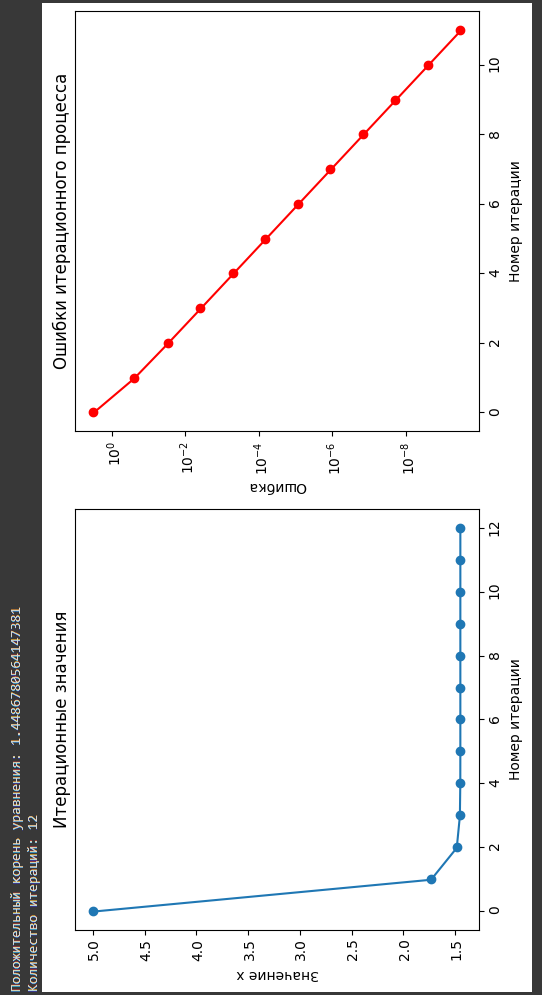
\includegraphics{iterations2.png}
		\caption{Результаты выполнения программы (см приложение [1])}
	\end{figure}
	\newpage
	\subsection{Приложение}
	[1] Код на python для расчетов 
	\begin{verbatim}
		import numpy as np
		import matplotlib.pyplot as plt
		
		# Функция итерационного процесса
		def phi(x):
		return (5 * x + 2) ** (1 / 6)
		
		# Параметры итерационного процесса
		x0 = 5.0  # Начальное приближение
		tolerance = 1e-9  # Допуск
		max_iterations = 100  # Максимальное количество итераций
		
		# Массивы для хранения значений
		x_values = [x0]
		errors = []
		
		# Итерационный процесс
		for n in range(max_iterations):
		x_next = phi(x_values[-1])
		x_values.append(x_next)
		error = abs(x_next - x_values[-2])
		errors.append(error)
		if error < tolerance:
		break
		
		# Печать результатов
		print(f"Положительный корень уравнения: {x_values[-1]}")
		print(f"Количество итераций: {len(x_values) - 1}")
		
		# Визуализация сходимости
		plt.figure(figsize=(10, 5))
		
		plt.subplot(1, 2, 1)
		plt.plot(x_values, marker='o')
		plt.title("Итерационные значения")
		plt.xlabel("Номер итерации")
		plt.ylabel("Значение x")
		
		plt.subplot(1, 2, 2)
		plt.plot(errors, marker='o', color='r')
		plt.yscale('log')
		plt.title("Ошибки итерационного процесса")
		plt.xlabel("Номер итерации")
		plt.ylabel("Ошибка")
		
		plt.tight_layout()
		plt.show()
		
	\end{verbatim}
		
		
	
\end{document}
